\documentclass[tikz,border=10pt]{standalone}
\usepackage{amsmath}
\usepackage{pgfplots}
\pgfplotsset{compat=1.18}
\definecolor{ink}{HTML}{21352F}
\definecolor{teal}{HTML}{087F7B}
\definecolor{blue}{HTML}{4B77A8}
\definecolor{gold}{HTML}{C58B2A}

\begin{document}
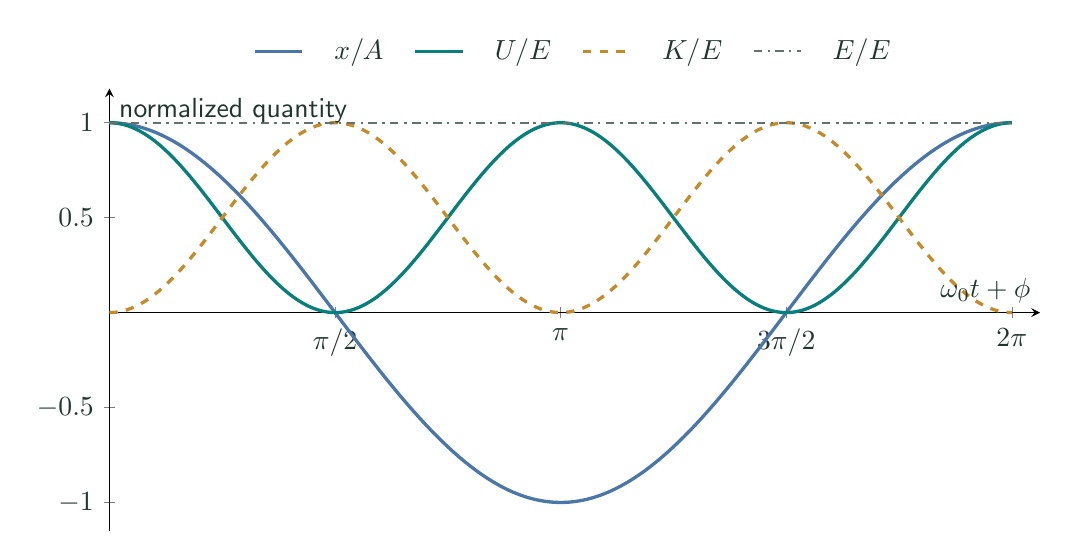
\begin{tikzpicture}[font=\sffamily,text=ink]
\begin{axis}[
  width=13.4cm,height=7.2cm,
  axis lines=middle,
  xmin=0,xmax=6.48,ymin=-1.15,ymax=1.18,
  xlabel={$\omega_0t+\phi$},ylabel={normalized quantity},
  xtick={0,1.570796,3.141593,4.712389,6.283185},
  xticklabels={$0$,$\pi/2$,$\pi$,$3\pi/2$,$2\pi$},
  ytick={-1,-.5,0,.5,1},
  legend style={at={(.5,1.03)},anchor=south,draw=none,
                legend columns=4,column sep=9pt},
  domain=0:6.283185,samples=260,clip=false
]
  \addplot[blue,very thick] {cos(deg(x))};
  \addlegendentry{$x/A$}
  \addplot[teal,very thick] {cos(deg(x))^2};
  \addlegendentry{$U/E$}
  \addplot[gold,very thick,dashed] {sin(deg(x))^2};
  \addlegendentry{$K/E$}
  \addplot[ink!70,thick,dash dot] {1};
  \addlegendentry{$E/E$}
\end{axis}
\end{tikzpicture}
\end{document}
